%!TEX root = ../main.tex

\newcommand{\fnaRetrievalTime}{\formatdate{25}{11}{2014} at \formattime{9}{14}{0}}

\chapter{Ribofinder}
\label{ch:rfinder}

\lhead{Ribofinder: A \Rb Detection Pipeline}

\section{Introduction}
\label{sec:rfinder:intro}

In this chapter, we present the \rfinder program---a pipeline to facilitate the
detection of putative \grbs across genomic data. The \rfinder
tool operates in three stages. First we use \infernal
\citep{infernal,nawrocki:2013hk} and \tthp \citep{ermolaeva:2000cl} to detect
putative aptamers and expression platforms, two distinct components of
\rbs described in \Secref{sec:rfinder:bkgrnd}. After coalescing
this data into a pool of candidate \rbs, we use \rfold \citep{lorenz.amb11}
with constraints based on experimental data to compute the two distinct structural
conformations---gene `on' and gene `off'. In the third and final stage, we
leverage \foldalign \citep{gorodkin:1997tr,havgaard:2007ca} to measure the similarity between our
candidate pool and a
canonical \grb well studied in the literature, the
xanthine phosphoribosyltransferase (xpt) \grb from {\em Bacillus subtilis}. At the
time of this writing, Prof. Dr. Mario
M\"orl at Universit\"at Leipzig is overseeing preliminary structural
validation of predicted gene `on' and `off' structures for a number of
computationally predicted \grbs in {\em Bacillus megaterium}. We have already
prepared a draft of the paper describing this work, and are presently awaiting
biochemical validation before submitting it with co-authors M. M\"orl and
coworkers.

\subsection{Organization}
\label{subsec:rfinder:org}

This chapter is organized in the following fashion. After providing background
on the structural components of a \rb alongside their biological
significance, we outline the deficiencies in the `state of the art' software
as it relates specifically to \rb detection. We then move on to outline
the three stages of \rfinder: candidate selection, structural prediction, and
candidate curation. Having described the approach of the software, we move on
to present our findings in using \rfinder to detect \grbs across
the bacterial RefSeq database. Finally, we provide brief commentary on possible
extensions of the algorithm to locate other flavors of \rbs, of which
adenine-sensitive aptamers are a straightforward extension.

\section{Background}
\label{sec:rfinder:bkgrnd}

\Rbs are regulatory mRNA elements that modulate gene expression via
structural changes induced by the direct sensing of a small-molecule metabolite.
Most often found in bacteria, \rbs regulate diverse pathways including the
metabolism and transport of purines, methionine, and thiamin amongst others. The
structure of a \rb includes an aptamer domain---involved in the direct
sensing of the small-molecule---and a downstream expression platform whose
structure changes upon the aptamer binding the metabolite. Because of the
discriminatory nature of metabolite sensing, groups have had great success in
finding representative examples of aptamers across a diverse collection of
bacterial species; Rfam $12.0$ currently contains $26$ different families of aptamers
involved in different metabolic pathways.

Tools such as \Rb finder \citep{bengert2004} and \ms{RiboSW}
\citep{chang:2009de} have used the conserved
structural characteristics of the aptamer as search criteria with promising
results, while the webserver \ms{RibEx} relies solely on sequence conservation
to detect putative aptamer domains in genomic data \citep{abreugoodger:2005hb}.
Meanwhile other groups have used covariance model (CM)-based approaches to find
aptamer domains, most notably \ms{CMfinder} \citep{yao2006} and Rfam
\citep{nawrocki:2014uy}.

Whereas there exists strong sequence and
structural similarity within the aptamer of a \rb family, the expression
platform is highly variable, and thus challenging to capture using traditional
SCFG-based approaches. For this reason databases such as Rfam only contain the aptamer
portion of the \rb, and there exists no database providing sequences
including expression platforms, necessary for capturing the `on' and `off'
conformations of this regulatory element. We have developed a new
pipeline---called \rfinder---which can detect putative \rbs including their
expression platforms and likely conformational structures across a wide collection
of genomic sequences.

\section{The \rfinder pipeline}
\label{sec:rfinder:pipeline}

At the time of our retrieval (\fnaRetrievalTime), the RefSeq database hosted by
NCBI comprised $5,121$ complete bacterial genomes with corresponding genomic
annotations. In order to both detect putative full \rbs across this
collection of data as well as filter the candidates down to a number tractable for
experimental validation, we developed a novel pipeline which takes a three-tiered
approach to candidate selection. Our approach is to
\begin{inparaenum}[\em 1\upshape)]
\item identify a pool of candidate \rbs across genomic data;
\item perform a coarse-grained filtering of the candidate pool based on structural
characteristics; and finally
\item fine-grained curation of the candidates based on a collection of measures
and pairwise similarity.
\end{inparaenum} \Figref{rfinder:flowchart} outlines this approach as a
flowchart.

\begin{figure}[!ht]
\centering
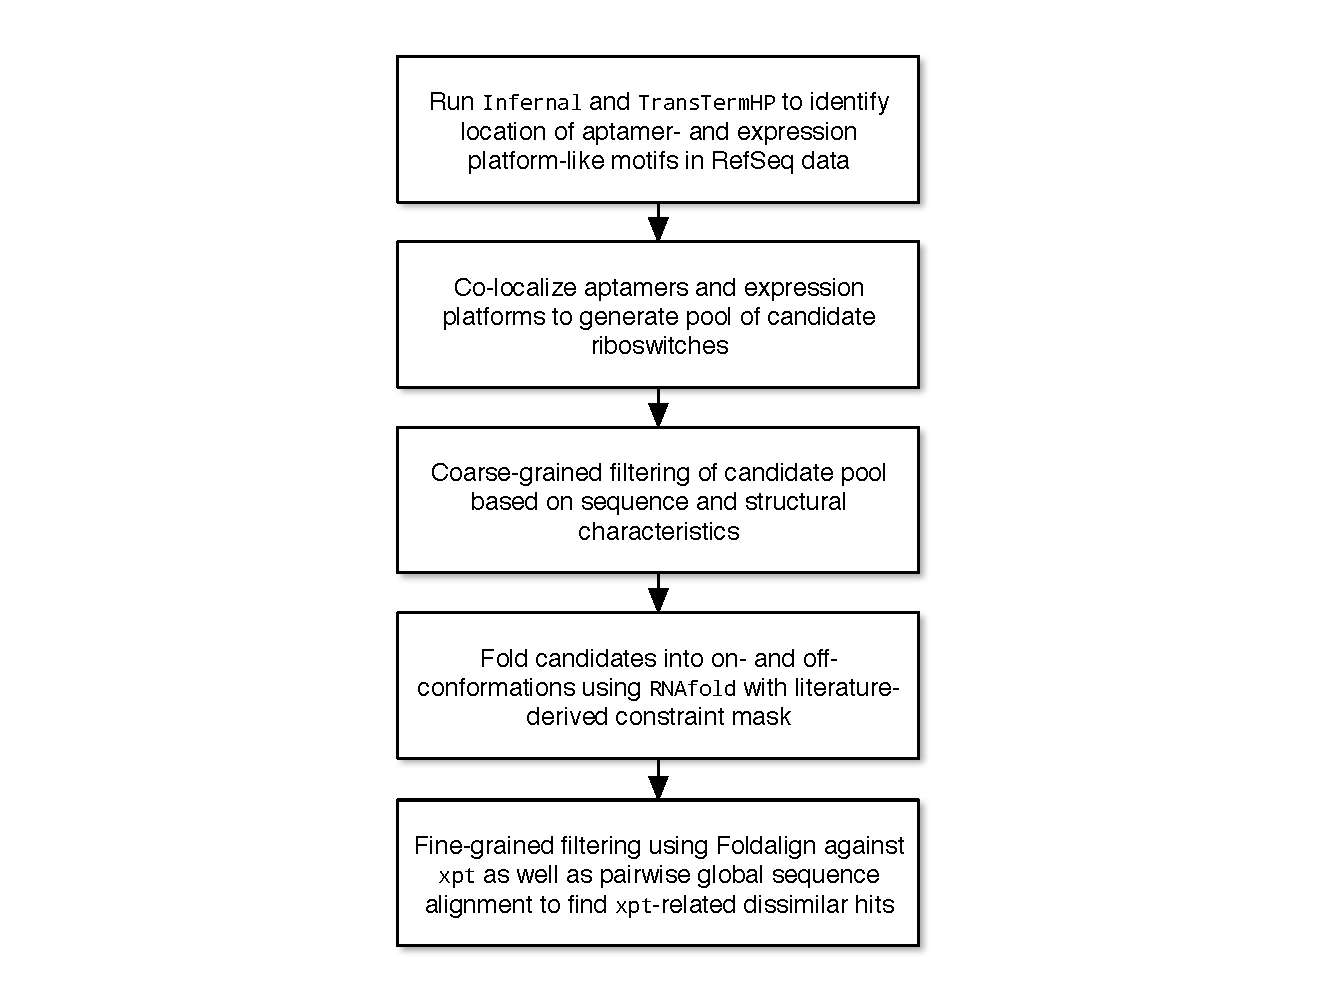
\includegraphics[width=.9\textwidth]{Figures/Ribofinder/ribofinderOverview.pdf}
\caption[Outline of the approach for the \rfinder pipeline]
{Outline of the approach for the \rfinder pipeline.}
\label{fig:rfinder:flowchart}
\end{figure}

In the following discussion, we describe the application of \rfinder to identify
unannotated guanine purine \rbs; guanine-sensing cis-regulatory elements
which modulate the expression of genes involved in purine biosynthesis.

\subsection{Step 1: Candidate selection}
\label{subsec:rfinder:selection}

The RefSeq data we used for analysis (downloaded on \fnaRetrievalTime)
contains $5,121$ annotated bacterial genomes
across $2,732$ different organisms, totaling over $9.5 \times 10^9$ bases. We used the
program \infernal to determine the coordinates of putative aptamer structures
within the RefSeq genomes, and \tthp to locate candidate rho-independent
transcription terminators.

\subsubsection{Detecting aptamers with \infernal}
\label{subsubsec:rfinder:infernal}

\infernal \citep{infernal,nawrocki:2013hk} uses a stochastic context-free
grammar (SCFG) with a user-provided multiple sequence alignment (MSA) to
efficiently scan genomic data for RNA homologs, taking into consideration both
sequence and structural conservation. Using the purine aptamer MSA from Rfam $12.0$
(RF$00167$), \infernal (v$1.1.1$, default options) detects $1,537$ significant hits
having E-value $<= 0.01$. Because \infernal leverages the concept of a
`local end'---a large insertion or deletion in the alignment at reduced cost---it
is possible for the software to return a significant hit whose aligned structure
does not have the canonical three-way junction observed in all purine
\rbs. \rfinder prunes these truncated \infernal hits by converting the
alignment structure into a parse tree, and only permitting trees of sufficient
complexity to contain a multiloop (described further in
\ref{subsubsec:rfinder:shapes}). The pyrimidine residue abutted next to the P1
stem in the J3--1 junction differentiates between guanine and adenine-sensing
\rbs by binding the complimentary purine ligand; for our interest in \grbs
exclusively we require the presence of a cytidine at this residue
(\Figref{rfinder:aptamerDiagram}). In total, using
\infernal with these additional filters yields $1,280$ guanine aptamers across $555$
unique organisms.

\begin{figure}[!ht]
\centering
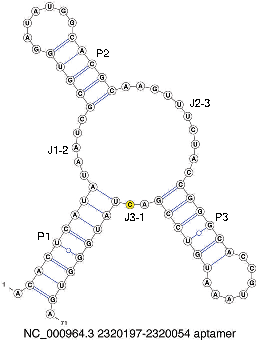
\includegraphics[width=.4\textwidth]{Figures/Ribofinder/NC_000964_3_2320197_2320054_APTAMER.pdf}
\caption[Diagram of the aptamer portion of the \Bsxpt \grb]{Diagram of the aptamer portion of the \Bsxpt \grb, with annotations
to indicate the P1, P2, and P3 stems of the multiloop, junctions between the
hairpins, and the ligand binding site (in yellow). This structural diagram was
generated using VARNA \citep{darty:2009gt}.}
\label{fig:rfinder:aptamerDiagram}
\end{figure}

\subsubsection{Detecting expression platforms with \tthp}
\label{subsubsec:rfinder:tthp}

\tthp \citep{ermolaeva:2000cl} detects rho-independent terminators in bacterial
genomes in a context-sensitive fashion by leveraging the protein annotations
available in NCBI Protein Table (PTT) data. These terminator sequences canonically have a stable
hairpin loop structure immediately preceding a run of $5+$ uracil residues, the
combination of which causes the ribosomal machinery to stall and dissociate from
the transcript. \tthp performs a genomic scan to determine candidate loci with
this motif, and returns scored hits. The scoring system considers both structural
homology and the genomic contextual information available in the PTT file. Across
our collection of bacterial genomes acquired from NCBI RefSeq data, \tthp
identified $2,752,469$ rho-independent terminators using the default filters.

Due to the spatially-mediated structural regulation of purine \rbs,
whereby ligand interaction with the aptamer domain induces local structural
rearrangement in the expression platform, we paired aptamers with corresponding
terminators by minimizing the genomic distance, with an upper bound of $200$
nucleotides between the end of the aptamer domain and start of the terminator.
This approach yields $577$ candidate \rbs, $81$ of which have multiple
rho-independent terminators within range of a putative aptamer produced by
\infernal. For these, we simply pair the closest \tthp hit with the aptamer domain.

\begin{figure}[!ht]
\centering
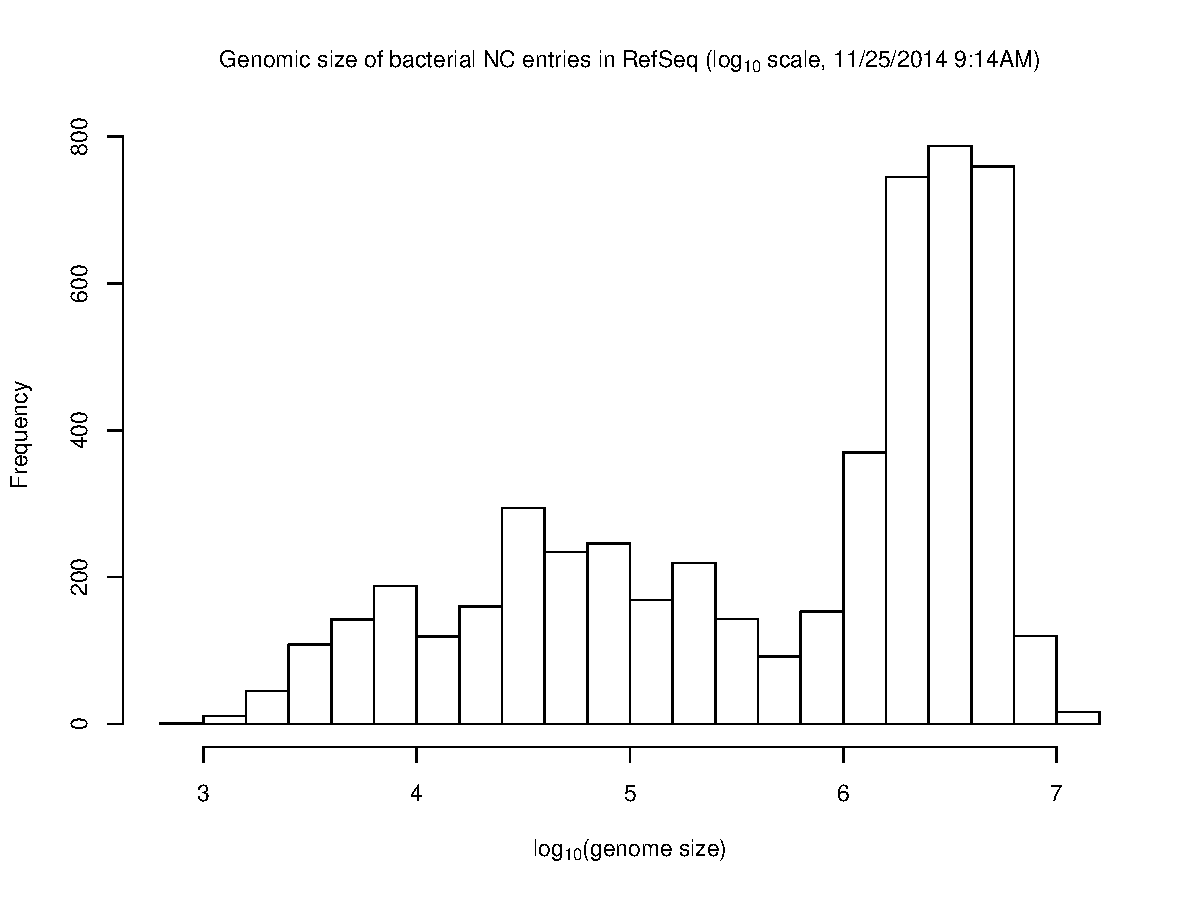
\includegraphics[width=.9\textwidth]{Figures/Ribofinder/refseqGenomeSizes.pdf}
\caption[Histogram displaying the distribution of genome sizes across RefSeq]{Histogram displaying the distribution of genome sizes across the RefSeq
data analyzed, comprising $5,172$ bacterial genomes. Genome size is shown using a
$\log_{10}$ scale, and appears to have a bimodal distribution.}
\label{fig:rfinder:genomeSizes}
\end{figure}

\subsection{Step 2: Structural prediction}
\label{subsec:rfinder:strpred}

Until this point we have been focused on the generation of candidate sequences
from our RefSeq dataset, without yet focusing on the specifics of underlying
secondary structures for these candidates. In the following section, we explain
how constraint folding is used to generate putative `on' and `off' conformations
for each candidate.

\subsubsection{Notation for representing abstract RNA shapes}
\label{subsubsec:rfinder:shapes}

Given an RNA sequence $\seq = \seqN$, where positions $s_i$ are drawn from the
collection of single-letter nucleotide codes, i.e.
$s_i \in \{\text{A,\,U,\,G,\,C}\}$, it is possible to describe a corresponding
secondary structure \strS compatible with \seq using the dot-bracket notation.
In this notation, each nucleotide $a_i$ has a corresponding state $s_i$, where
$s_i$ is denoted as a `.' if unpaired and a `(' [resp. `)'] if the left [resp.
right] base in a base pair. Given any two base pairs $(i,j)$ and $(k,l)$ in \strS,
then $i < k < j \iff i < l < j$; pseudoknots are not permitted in the structure. A
secondary structure taking this form is said to have balanced parentheses, and can
additionally be represented using a context-free grammar such as the
following, derived from \citep{fusy:2012ka}:

\begin{align}
\label{eq:rfinder:strCfg}
S &\rightarrow \bullet \;|\; S \bullet \,|\; \bpL S \bpR \;|\; S\, \bpL S \bpR
\end{align}

The grammar from \eqnref{rfinder:strCfg},
where the minimum number of unpaired bases $\theta$ in a hairpin loop
is taken to be $1$ for expository clarity,
can be used to generate a parse tree
\tree for \strS. The benefit of working with \tree over \strS is that the parse
tree offers an abstract representation of secondary structure shape independent of
sequence length, permitting us to classify and eventually constrain a large
collection of sequences having variable length which are all expected to have the
same abstract tree shape \citep{voss:2006iq}. This is analogous to what
the Giegerich lab refers to as
their `type 5' structural abstraction using the \rshapes tool, and can be
described using the following grammar \citep{Lorenz:2008gz}, which generates
all combinations of matched brackets:

\begin{align}
\label{eq:rfinder:shapeCfg}
\begin{split}
S &\rightarrow \brL T \brR\, S \;|\; \brL T \brR \\
T &\rightarrow \brL T \brR \;|\; \epsilon \\
\end{split}
\end{align}

Every node in \tree
represents a helix in \strS, and internally tracks the indices of both its
beginning $(i,j)$ and closing $(k,l)$ base pair. We use a level-order naming
convention to refer to helices within the parse tree, whereby a position
\treePos{p}{1} references the first child of the root node, \treePos{p}{1,2}
references the second child of \textdown{\ms{p}}{1}, and generally
\treePos{p}{$i_1,i_2,\cdots,i_n$} refers to the $i_n$\textsuperscript{th} child of
\treePos{p}{$i_1,i_2,\cdots,i_{n-1}$}. To reference specific nucleotides in the
context of their location relative to a helix, we use the opening and closing base
pairs $(i,j)$ and $(k,l)$ as landmarks. Thus, \treeIdx{p}{1}{l} is the index in
\strS of the right-hand side closing base pair of \treePos{p}{1}. We use the
notation \treePos{t}{$i$} to refer to the subtree of \tree whose root is
\treePos{p}{$i$}.

Finally, we introduce the concept of a tree signature. The tree signature for a
tree \tree is a list of the node depths when traversed in a depth-first pre-order
fashion. To provide a concrete example, consider the following experimentally
validated xpt \grb from {\em Bacillus subtilis} subsp. subtilis str. $168$
(NC\_$000964.3$ $2320197$--$2320054$) with corresponding gene `off' structure as seen in
\Figref{rfinder:xptOff}.
\medskip

\begin{figure}[!ht]
\centering
\begin{subfigure}[h]{\textwidth}
\centering
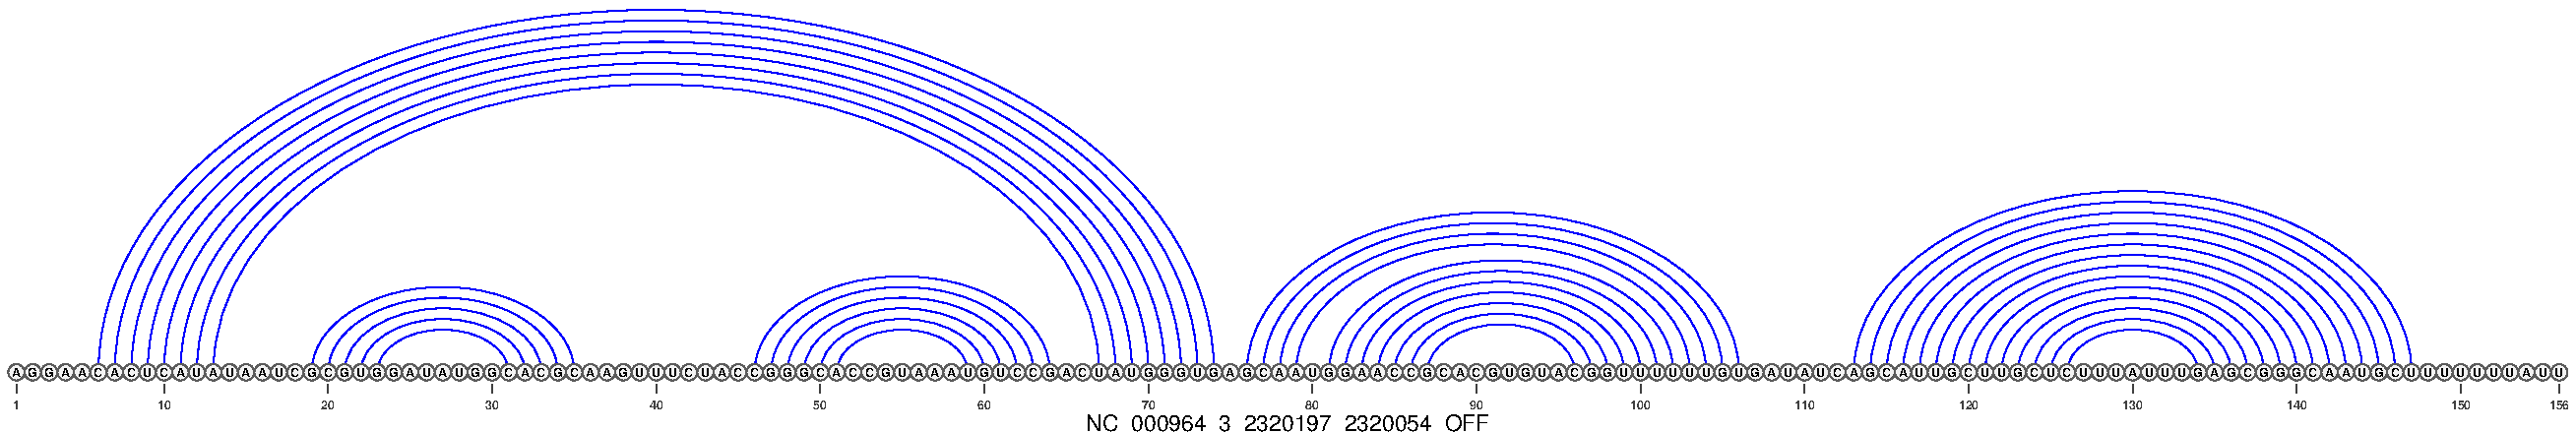
\includegraphics[width=.9\textwidth]{Figures/Ribofinder/NC_000964_3_2320197_2320054_OFF.pdf}
\end{subfigure} \\
\medskip
\begin{subfigure}[h]{\textwidth}
\centering
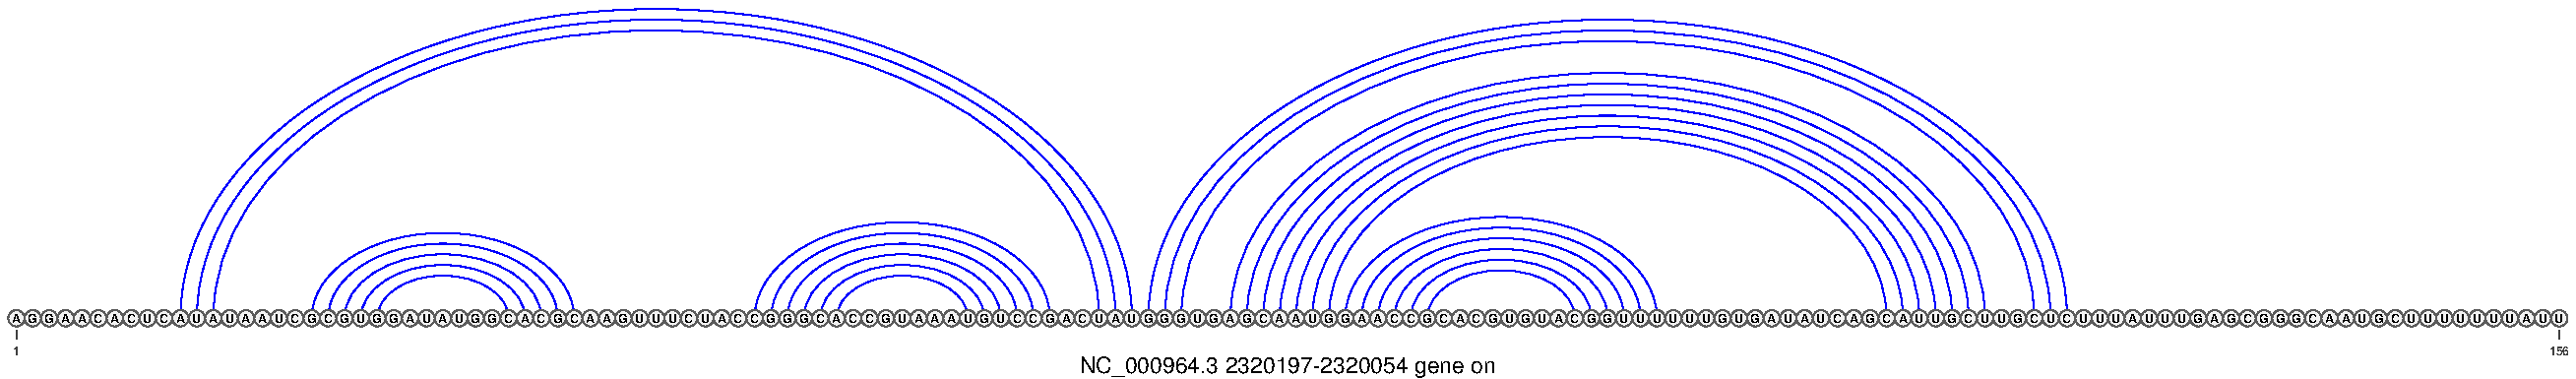
\includegraphics[width=.9\textwidth]{Figures/Ribofinder/NC_000964_3_2320197_2320054_ON.pdf}
\end{subfigure}
\caption[The xanthine phosphoribosyltransferase (xpt) \grb from
{\em B. subtilis} subsp. subtilis str. $168$ (NC\_$000964.3$ $2320197$--$2320054$),
and corresponding gene `off' and `on' structures]{{\em (Top)} The xanthine phosphoribosyltransferase (xpt) \grb from
{\em B. subtilis} subsp. subtilis str. $168$ (NC\_$000964.3$ $2320197$--$2320054$),
and corresponding gene `off' structure derived from inline probing studies both in
the presence and absence of guanine \citep{mandal2003}. {\em (Bottom)} The
experimentally
derived gene `on' structure for \Bsxpt. These structural diagrams were generated
using VARNA \citep{darty:2009gt}.}
\label{fig:rfinder:xptOff}
\end{figure}

The \rshapes \citep{janssen:2015cq} `type 5' representation for this structure is
\ms{[[][]][][]} (note the coalesced left bulge in the hairpin immediately
downstream the closing multiloop stem, at helix \treePos{p}{2}) and the tree
signature for this parse tree of the structure is \ms{[0,1,2,2,1,1]}.

We leverage the notion of abstract structural filtering initially to ensure that
all \infernal aptamer hits have a tree signature of \ms{[0,1,2,2]}, which
represents a three-way junction, and that the binding site for the guanine ligand
$\treeIdx{p}{1}{l - 1} = \text{C}$. These filters, in combination with the
proximal terminator hairpins produced by \tthp yield the aforementioned $577$
candidate \grbs for which we then try to produce reasonable gene `on' and off
structures.

\subsubsection{Constrained folding to predict switch structures}
\label{subsubsec:rfinder:consfold}

To restrict our search to unannotated \grbs, and further ensure that we are not
re-detecting sequences based off the Rfam covariance model provided to \infernal,
we constrain our search to those RefSeq organisms not represented in the Rfam seed
alignment. $503$ of the $577$ candidates, or $87.18$\% represent putative unannotated
\rbs not represented by RF$00167$.

The gene `off' structure \strOff for a \grb is the easier of the two to find
computationally, since the terminator stem is exceptionally thermodynamically
stable. In the gene `on' conformation \strOn, the P1 stem of the multiloop partially
dissociates and an anti-terminator stem forms between the region immediately 3' of
the P1 stem and what was the left-hand side of the terminator stem. This truncated
P1 stem, which closes the three-way junction in the aptamer, is exceptionally
unstable based on present energy models available for structural folding, and
requires special treatment to reconstitute in our final structures.

The software \rfold (v$2.1.8$) allows for the folding of RNA molecules with `loose'
constraints. In this model of constrained folding, the resulting structure
produced by the software guarantees not to explicitly invalidate any user-provided
constraints, but does not guarantee all constraints will be satisfied in the
resulting structure. For each of the candidate \grbs, having \treeFor{\infernal}
and \treeFor{\tthp}, we build the following constraint masks:

{\large Structural constraints for both conformations of the \grb aptamer:}
\begin{enumerate}
\setstretch{1.3}
\item Prohibit base pairing upstream of \treeIdx{p}{1}{i} and
downstream of \treeIdx{p}{2}{l}. \\[1.5ex] {\em Do not permit any possible disruptive pairing
interactions 5' of the aptamer or 3' of the terminator stem.}
\item Force base pairs and unpaired regions in \treePos{t}{1}, with
the exception of \treePos{p}{1}. \\[1.5ex] {\em Since the aptamer structure is well
conserved and we have the \infernal-provided alignment with the
covariance model, force this structure to form as aligned.}
\item Explicitly prohibit formation of \treePos{p}{1} stem, which closes the
three-way junction. \\[1.5ex] {\em The only exception to above is the closing of the
P1 multiloop stem. In our experience, since \rfold uses soft constraints
(meaning that constrained base pairs are only allowed to pair with each other
or not at all), in practice we rarely see the P1 stem form as we would like.
Instead, restrict it from forming at all, so that it can be added in after the
fact without disrupting any other base pairs.}
\end{enumerate}
{\large Constraints exclusive to the gene `off' structure:}
\begin{enumerate}
\setstretch{1.3}
\item Force base pairs and unpaired regions in \treePos{t}{2}. \\[1.5ex] {\em This simply
forces the formation of the terminator stem, as predicted by \tthp.}
\end{enumerate}
{\large Constraints exclusive to the gene `on' structure:}
\begin{enumerate}
\setstretch{1.3}
\item Require $m$ nucleotides starting from \treeIdx{p}{1}{l + 3} to pair to the
right, where $m = \textit{length}(\treePos{p}{2})$, and require the left-hand side of the
\treePos{p}{2} helix to pair to the left. \\[1.5ex] {\em The formation of the
anti-terminator stem involves the partial disruption of the \treePos{p}{1} stem.
Though there is no consensus for the length of the anti-terminator stem,
experimental data suggests that the left side of the terminator stem}
(\treeIdx{p}{2}{i}--\treeIdx{p}{2}{k}) {\em alternatively base pairs to the left,
thus forming the anti-terminator hairpin and permitting transcription to proceed
\citep{mandal:2004ja}.}
\item Disallow pairing downstream of \treeIdx{p}{2}{j}. \\[1.5ex] {\em Avoid
disruptive pairing downstream of the newly formed anti-terminator stem.}
\end{enumerate}

These constraint masks are run using the command-line flags
\ms{-d 0 -P rna\_turner1999.par} to disable dangles and use the Turner $1999$
energies respectively \citep{mathews:1999jw}. We choose to disable dangles (\ms{-d 0}) and use
the Turner $1999$ energy model (\ms{-P rna\_turner1999.par})
based on visual inspection of the structures output by \rfold with
constraints---these flags appear to yield conformations most frequently consistent
with the known structures for the \Bsxpt \grb.
Experimental evidence using inline probing and
crystallographic analysis suggests that
the `on' conformation of the \grb has a reduced P1 stem length of $3$ base pairs
\citep{mandalboesebarrickwinklerbreaker,serganov:2004dq};
in practice we were unable to force \rfold to respect this constraint regardless
of command-line options specified. For this reason we reconstitute the P1 stem in
both structures after constrained folding, having length equivalent to it the
\infernal P1 stem [resp. $3$ base pairs] in the gene `off' [resp. gene `on']
structure.

\subsection{Step 3: Candidate curation}
\label{subsec:rfinder:curation}

Until now, we have described our approach for generating the $503$ \grb candidates
in RefSeq, alongside their gene `on' and off structures. Unfortunately the
experimental validation of all $503$ candidates is not tractable, so it was
necessary to reduce this collection again to a more manageable size, while only
keeping the most promising candidates. Our original approach involved using
\foldalign \citep{gorodkin:1997tr,havgaard:2007ca} alongside the \ms{needleall} tool from EMBOSS
\citep{rice:2000wr}, to simultaneously
select sequences which closely approximate the more thermodynamically stable
gene `off' conformation of the experimentally known \Bsxpt \grb, while minimizing
sequence similarity between candidates selected for experimental validation. Due to
expense, we elected to instead choose a small number
($n = 2$) of organisms easily available which had multiple promising hits as our
experimental candidate pool.

In \Figref{rfinder:histogramFoldalignCandidatesVsXpt}, we display a histogram of scores produced
by \foldalign for the $503$ candidates, when aligned with the \Bsxpt \grb. \foldalign
is based off a simplification of Sankoff's algorithm \citep{sankoff:1985wc}, and
is a dynamic programming
algorithm for simultaneous folding and alignment that runs in \On{4} time. Because three of the sequences from our pool of $503$ candidates have
no global alignment with the \Bsxpt sequence, we have pruned them from our
dataset and only consider those remaining $500$ sequences for which \foldalign
scores are produced. The \foldalign scores produce have a mean of $153.798$ with a
minimum [resp. maximum] score of $-2698$ [resp. $1908$]. Running \foldalign with the
\Bsxpt sequence aligned with itself produces a theoretical maximum score of $2419$.

\begin{figure}[!ht]
\centering
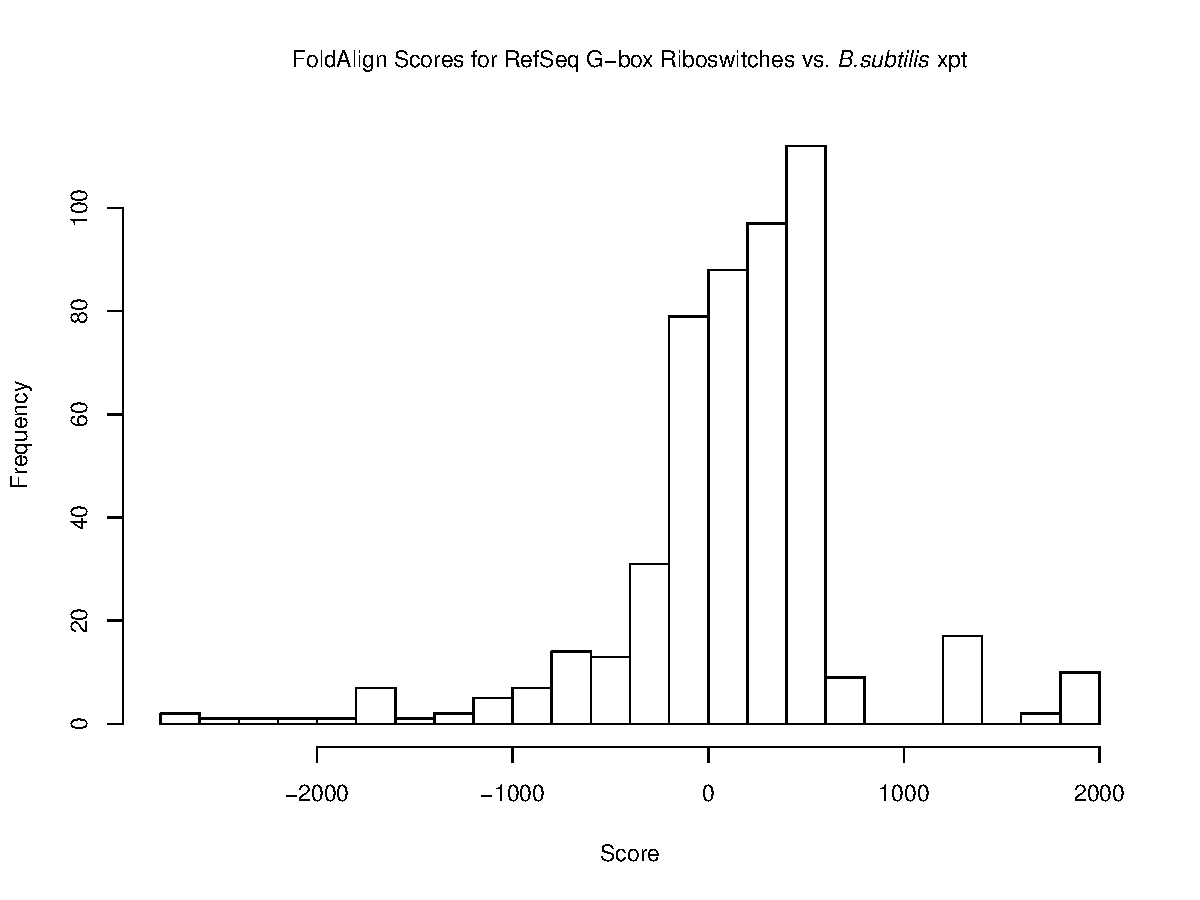
\includegraphics[width=.9\textwidth]{Figures/Ribofinder/histogramFoldalignCandidatesVsXpt.pdf}
\caption[Histogram displaying the distribution of scores produced by \foldalign]{Histogram displaying the distribution of scores produced by \foldalign
$2.1.1$ using flags \ms{-global -summary -format commandline} when folding each of
the $503$ candidates against the \Bsxpt sequence NC\_$000964.3$ $2320197$--$2320054$.
Three of the sequences run against \foldalign (NC\_$010674.1$ $1516712$--$1516868$,
NC\_$010723.1$ $1487041$--$1487197$, and NC\_$020291.1$ $4599412$--$4599258$) have no global
alignment with the \Bsxpt sequence, and thus the histogram represents $500$ of the
original $503$ sequences.}
\label{fig:rfinder:histogramFoldalignCandidatesVsXpt}
\end{figure}

Of these $500$ sequences, $335$ have a \foldalign score $s > 0$, representing $227$
unique accession numbers, with a distribution of candidates per accession number
as shown in \Figref{rfinder:candidateHistogramGroupedByAccession}. From
the perspective of experimental validation, we have tried to maximize the chance
of success per organism by selecting those having multiple candidates within the
same genome. Only $25$ of the candidate organisms have more than three hits within
their genome (only two have five hits). Our approach for selecting the initial
two organisms for experimental validation was to take this pool of $25$ organisms,
sort by descending average score $s$, and select the first two which are available
via DSMZ (\url{https://www.dsmz.de/}), the warehouse for microorganisms used by
our collaborators. Prof. Dr. Mario M\"orl at Universit\"at Leipzig is presently
overseeing Dr. Regula Aregger, a post-doc who is using the SHAPE protocol
\citep{wilkinson:2006vd} to
validate the computationally predicted structure of these candidates.

\begin{figure}[!ht]
\centering
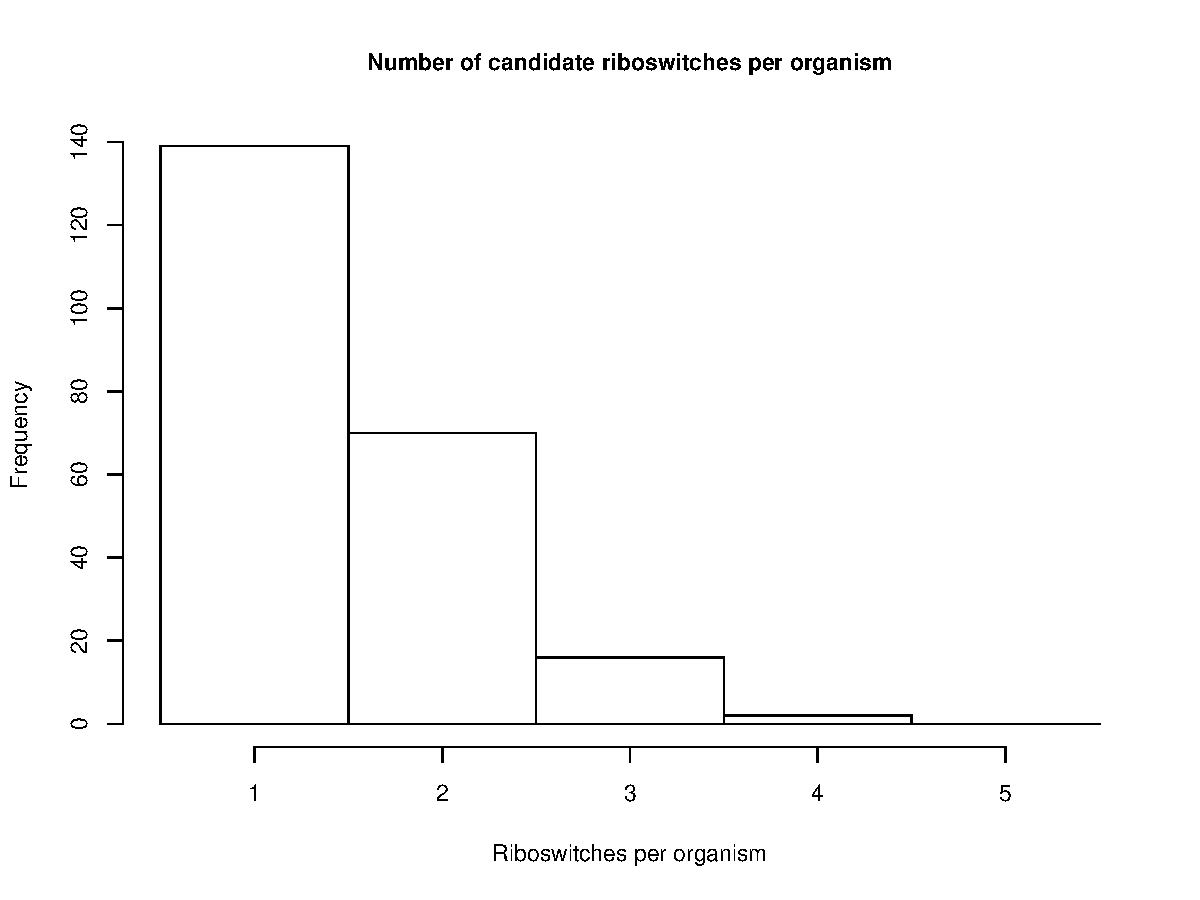
\includegraphics[width=.9\textwidth]{Figures/Ribofinder/candidateHistogramGroupedByAccession.pdf}
\caption[Histogram displaying the number of candidate \rbs we observe
per organism]{Histogram displaying the number of candidate \rbs we observe
per organism. From this data, it is clear that the majority of organisms have
only one putative \rb, however two organisms have five candidates each:
{\em Clostridium botulinum} B str. Eklund $17$B (NC\_$010674.1$) and
{\em Clostridium botulinum} E3 str. Alaska E$43$ (NC\_$010723.1$)}
\label{fig:rfinder:candidateHistogramGroupedByAccession}
\end{figure}

Proceeding in this fashion, we have selected {\em B. megaterium} QM B$1551$
(\href{http://www.ncbi.nlm.nih.gov/nuccore/NC_014019.1}{NC\_$014019.1$},
\href{http://www.dsmz.de/catalogues/details/culture/DSM-1804.html}{DSM$1804$})
and {\em B. megaterium} DSM$319$
(\href{http://www.ncbi.nlm.nih.gov/nuccore/NC_014103.1}{NC\_$014103.1$},
\href{http://www.dsmz.de/catalogues/details/culture/DSM-319.html}{DSM$319$})
for initial validation. These organisms have four
candidate \grbs each, outlined in Table \ref{table:rfinderCandidateLocs}.

\begin{table}[!ht]
\centering
\begin{tabularx}{\linewidth}{*{1}{L} *{2}{C}}
\toprule
\small{Downstream gene function} & \small{{\em B. megaterium} QM B$1551$} & \small{{\em B. megaterium} DSM$319$} \\
\cmidrule(lr){1-3}
\small{xpt} & $1427313$--$1427501$ & $1413696$--$1413884$ \\[1ex]
\small{GMP synthase} & $231630$--$231806$ & $230059$--$230235$ \\[1ex]
\small{guanine permease} & $233482$--$233680$ & $231911$--$232108$ \\[1ex]
\small{N5-carboxyaminoimidazole} & $240759$--$240970$ & $239188$--$239400$ \\
\bottomrule
\end{tabularx}
\caption[The genomic coordinates for the four candidate \grbs in both
{\em B. megaterium} QM B$1551$ and {\em B. megaterium} DSM$319$]{The genomic coordinates for the four candidate \grbs in both
{\em B. megaterium} QM B$1551$ and {\em B. megaterium} DSM$319$. Note that the
\grbs are located upstream of the same genes, and that these two strains of
{\em B. megaterium} are highly similar. These structures are pictured in
\Secref{sec:rfinder:grbValidationVarna}, plotted using VARNA \citep{darty:2009gt}.}
\label{table:rfinderCandidateLocs}
\end{table}

\section{Extending beyond \grbs}
\label{sec:rfinder:ext}

We believe that the \rfinder pipeline allows for the detection of both structural
conformations of \rbs beyond the \grb. The investigation of
adenine-sensitive purine \rbs is a small extension of the existing
implementation. As indicated in \Secref{subsubsec:rfinder:infernal}, adenine
\rbs have a complimentary uradine residue at the ligand binding site in
the J3--1 junction within the aptamer. Beyond differences in ligand specificity,
the adenine \rb anti-terminator stem is incorporated into the aptamer structure
itself, and thus stabilized with the base pairing of the adenine ligand. As a
result, the adenine \rb permits transcription when bound, unlike the \grb.
As a result of the extensive overlap between the anti-terminator stem and adenine
\rb aptamer, the formation of the terminator stem completely dissociates both the
P3 and P1 stems \citep{mandal2004a}.

From a computational perspective, these changes are simple to handle within the
\rfinder pipeline, and provide some indication to how we believe the framework
could be more generally applied in the future. Rather than filter for the
discriminatory cytidine residue in the \rb aptamer (\Secref{subsubsec:rfinder:infernal}) we can only select those hits from \infernal having a uridine at the
ligand binding site. Structural on and off conformations are known from
experimental data for the {\em B. subtilis} ydhL gene \citep{mandal2004a} and can
be used as templates for the constraint masks used in \Secref{subsec:rfinder:strpred}.

In general, we believe those \rbs using rho-independent transcription
termination as a mode of regulation---for which an aptamer alignment exists and
some experimental knowledge of the expression platform's structural
conformation is known---are well suited for more robust structural
prediction using \rfinder.

\section{Guanine \rbs for experimental validation}
\label{sec:rfinder:grbValidationVarna}

\begin{figure}[!ht]
\centering
\begin{subfigure}[h]{\textwidth}
\centering
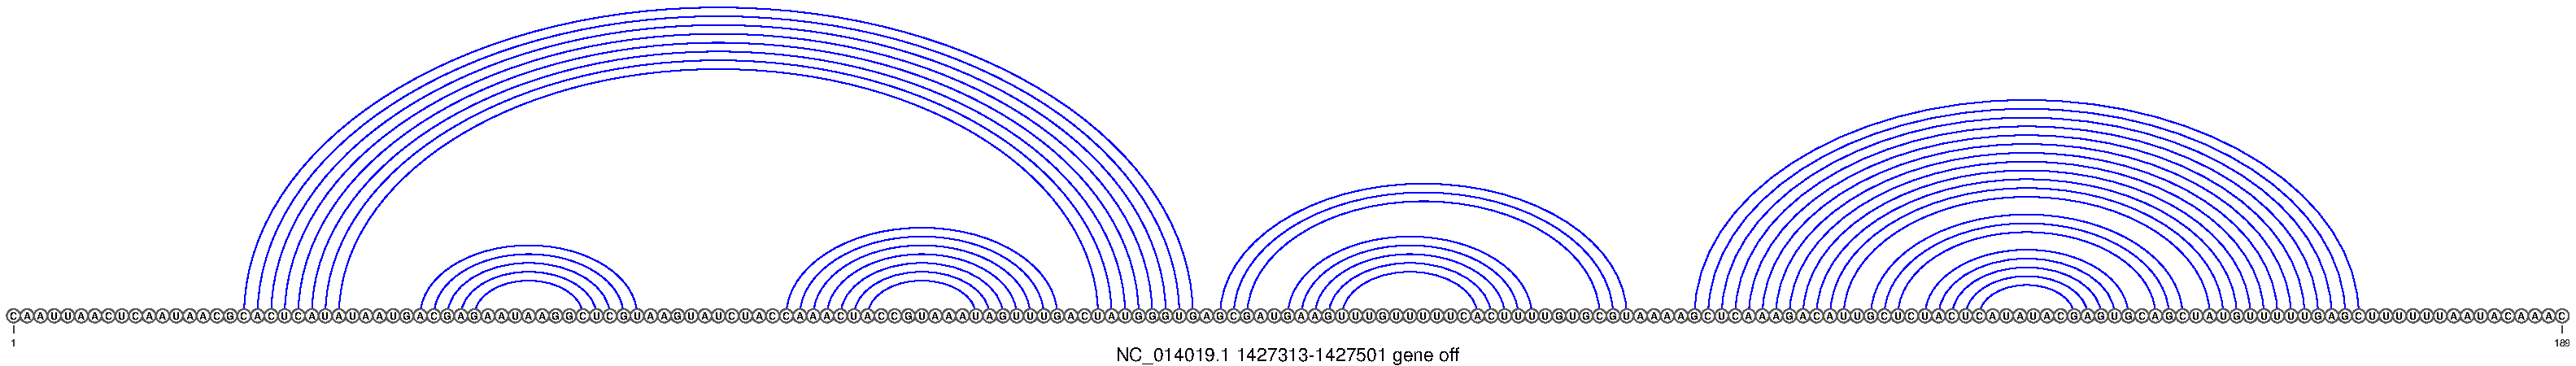
\includegraphics[width=.9\textwidth]{Figures/Ribofinder/NC_014019_1_1427313_1427501_OFF.pdf}
\end{subfigure} \\
\medskip
\begin{subfigure}[h]{\textwidth}
\centering
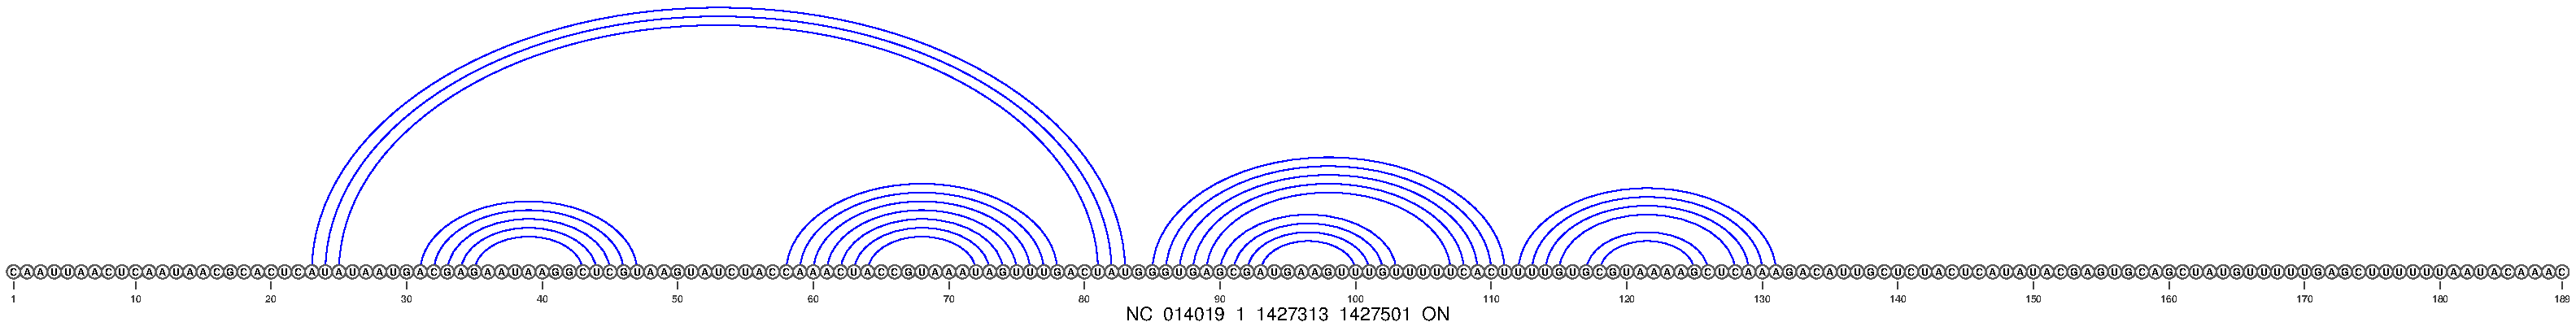
\includegraphics[width=.9\textwidth]{Figures/Ribofinder/NC_014019_1_1427313_1427501_ON.pdf}
\end{subfigure}
\caption[Structures for the putative \rb located upstream of the xpt gene in {\em B. megaterium} QM B$1551$]{{\em Top:} the computationally predicted gene `off' conformation of
sequence NC\_$014019.1$ $1427313$--$1427501$, using \rfold from the ViennaRNA $2.1.8$
suite, with dangles disabled and the Turner $1999$ energies. This sequence is
located upstream of the xpt gene in {\em B. megaterium} QM B$1551$. {\em Bottom:}
the gene `on' conformation.}
\label{fig:figure:NC_014019_1_1427313_1427501}
\end{figure}
\medskip

\begin{figure}[!ht]
\centering
\begin{subfigure}[h]{\textwidth}
\centering
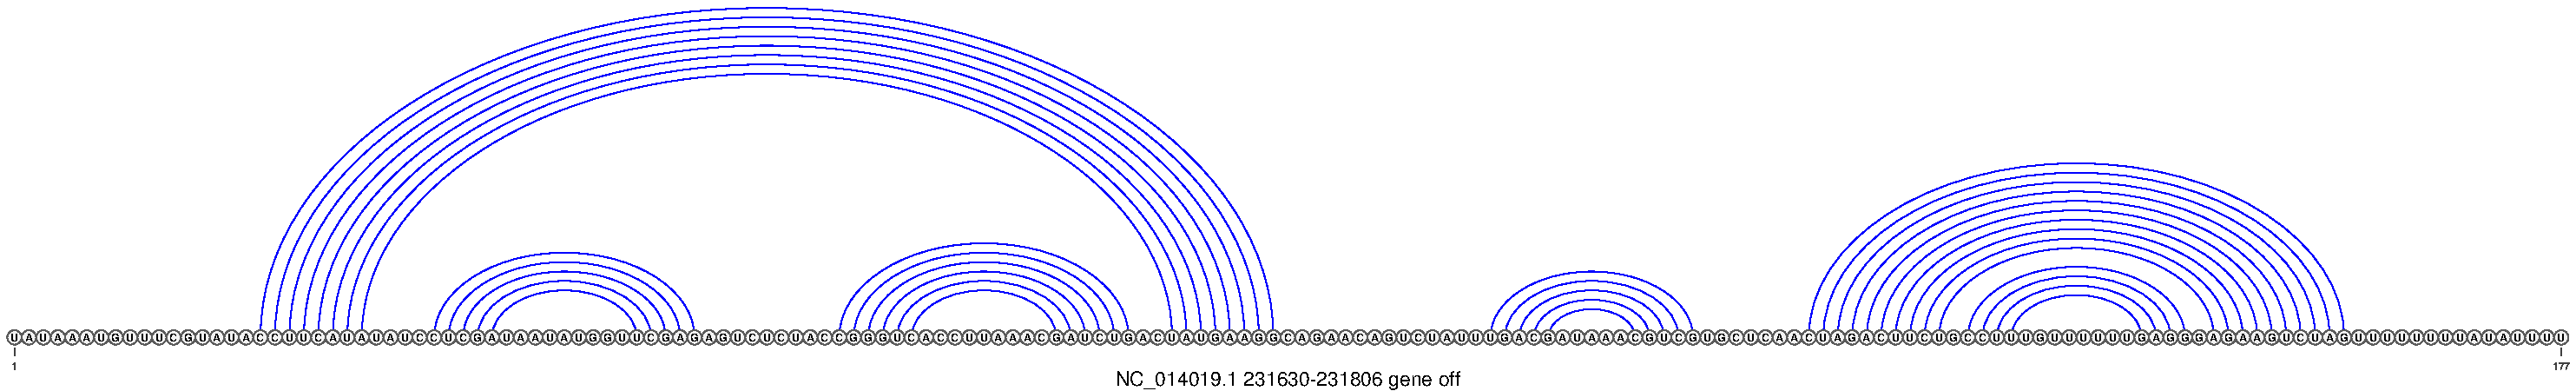
\includegraphics[width=.9\textwidth]{Figures/Ribofinder/NC_014019_1_231630_231806_OFF.pdf}
\end{subfigure} \\
\medskip
\begin{subfigure}[h]{\textwidth}
\centering
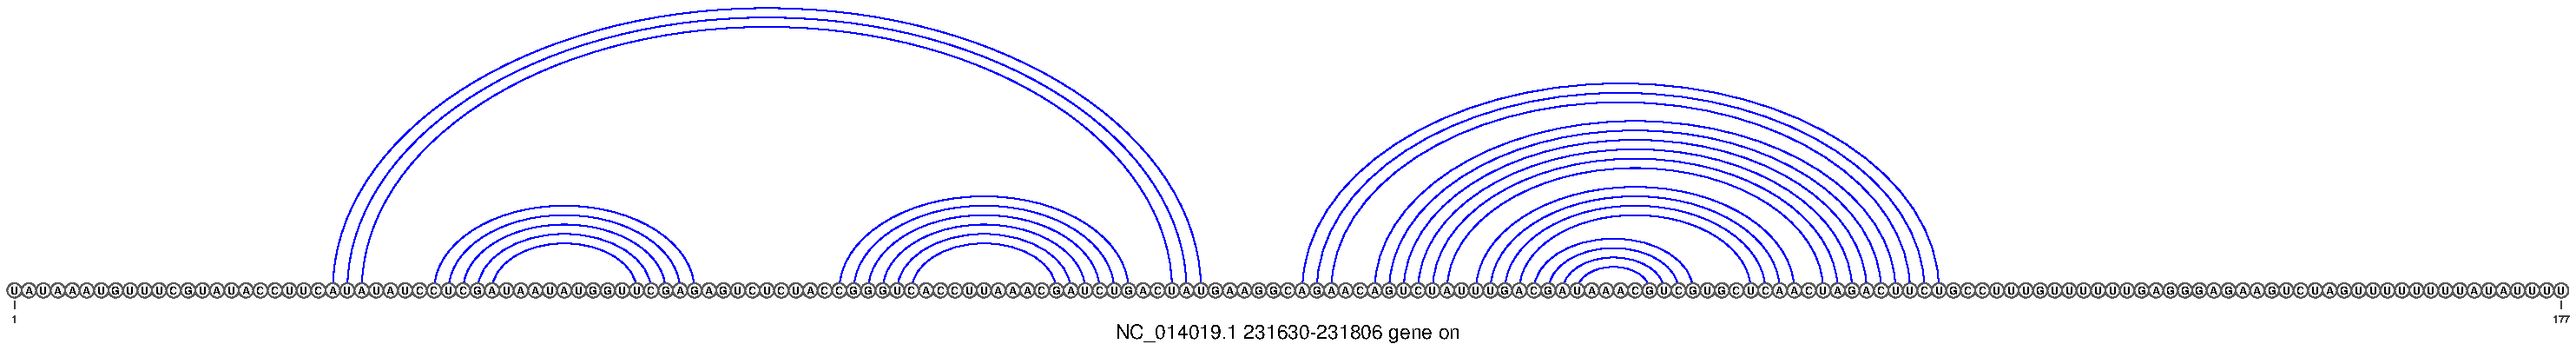
\includegraphics[width=.9\textwidth]{Figures/Ribofinder/NC_014019_1_231630_231806_ON.pdf}
\end{subfigure}
\caption[Structures for the putative \rb located upstream of the GMP synthase gene in {\em B. megaterium} QM B$1551$]{The computationally predicted \rb located upstream of the GMP synthase
gene in {\em B. megaterium} QM B$1551$ (NC\_$014019.1$ $231630$--$231806$).
{\em Top:} The gene `off' conformation. {\em Bottom:} The gene `on' conformation.}
\label{fig:figure:NC_014019_1_231630_231806}
\end{figure}
\medskip

\begin{figure}[!ht]
\centering
\begin{subfigure}[h]{\textwidth}
\centering
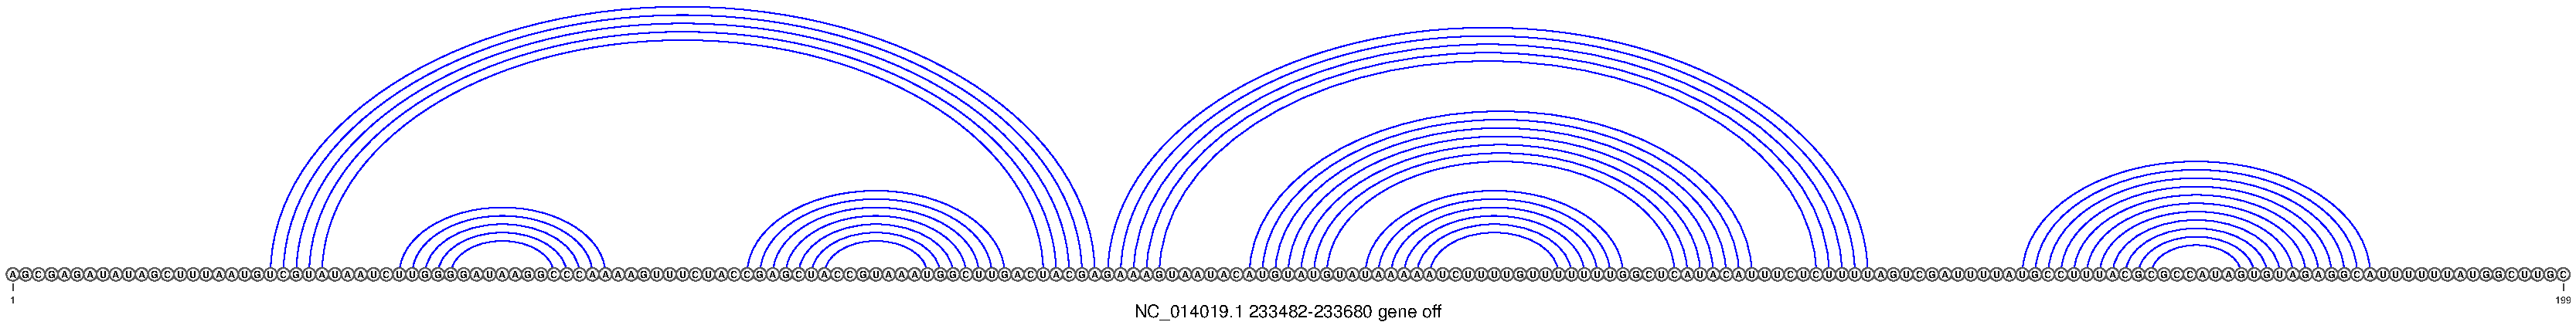
\includegraphics[width=.9\textwidth]{Figures/Ribofinder/NC_014019_1_233482_233680_OFF.pdf}
\end{subfigure} \\
\medskip
\begin{subfigure}[h]{\textwidth}
\centering
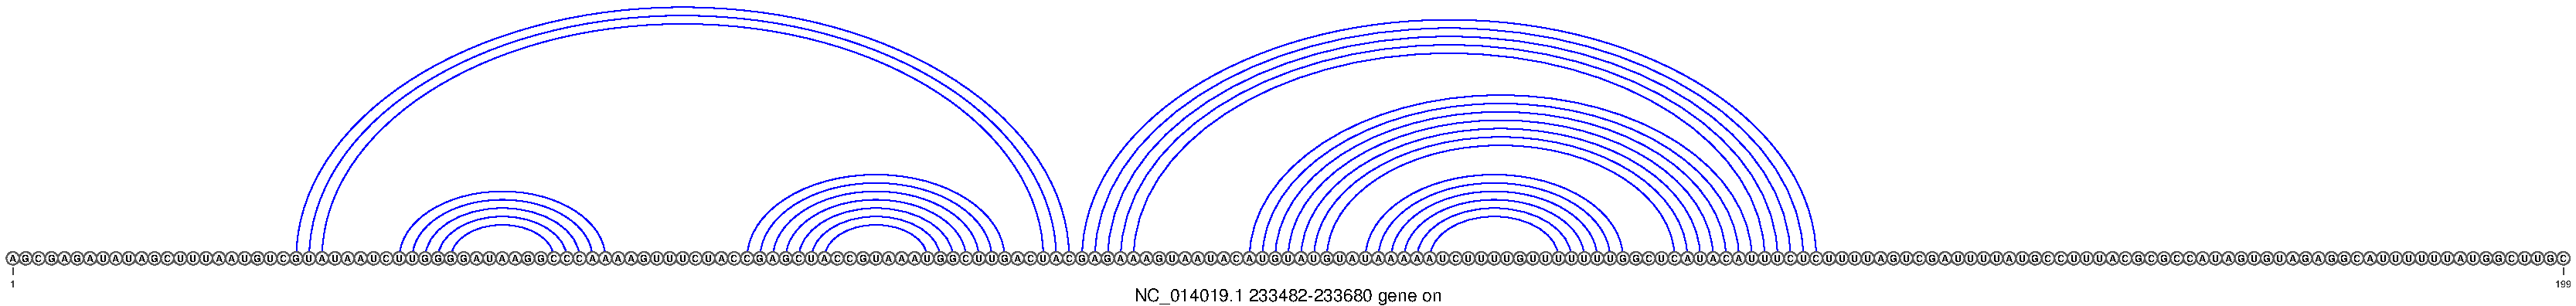
\includegraphics[width=.9\textwidth]{Figures/Ribofinder/NC_014019_1_233482_233680_ON.pdf}
\end{subfigure}
\caption[Structures for the putative \rb located upstream of the guanine permease gene in {\em B. megaterium} QM B$1551$]{The computationally predicted \rb located upstream of the guanine permease
gene in {\em B. megaterium} QM B$1551$ (NC\_$014019.1$ $233482$--$233680$).
{\em Top:} The gene `off' conformation. {\em Bottom:} The gene `on' conformation.}
\label{fig:figure:NC_014019_1_233482_233680}
\end{figure}
\medskip

\begin{figure}[!ht]
\centering
\begin{subfigure}[h]{\textwidth}
\centering
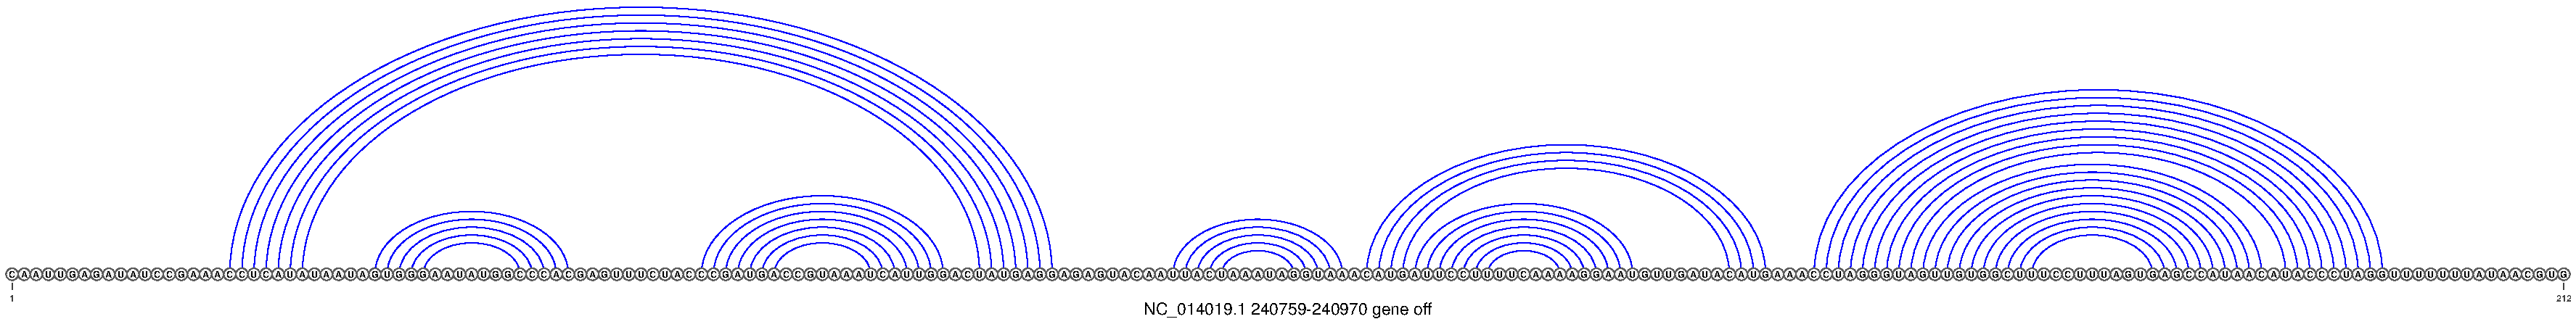
\includegraphics[width=.9\textwidth]{Figures/Ribofinder/NC_014019_1_240759_240970_OFF.pdf}
\end{subfigure} \\
\medskip
\begin{subfigure}[h]{\textwidth}
\centering
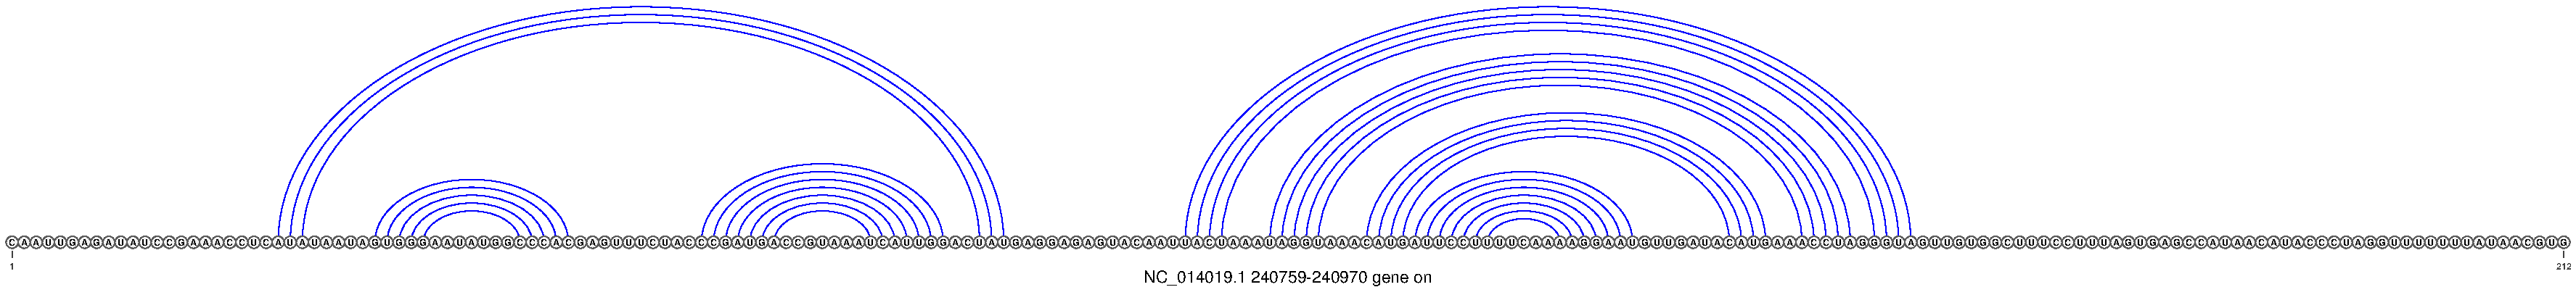
\includegraphics[width=.9\textwidth]{Figures/Ribofinder/NC_014019_1_240759_240970_ON.pdf}
\end{subfigure}
\caption[Structures for the putative \rb located upstream of the N5-carboxy\-amino\-imidazole gene in {\em B. megaterium} QM B$1551$]{The computationally predicted \rb located upstream of the
N5-carboxy\-amino\-imidazole
gene in {\em B. megaterium} QM B$1551$ (NC\_$014019.1$ $240759$--$240970$).
{\em Top:} The gene `off' conformation. {\em Bottom:} The gene `on' conformation.}
\label{fig:figure:NC_014019_1_240759_240970}
\end{figure}
\medskip

\begin{figure}[!ht]
\centering
\begin{subfigure}[h]{\textwidth}
\centering
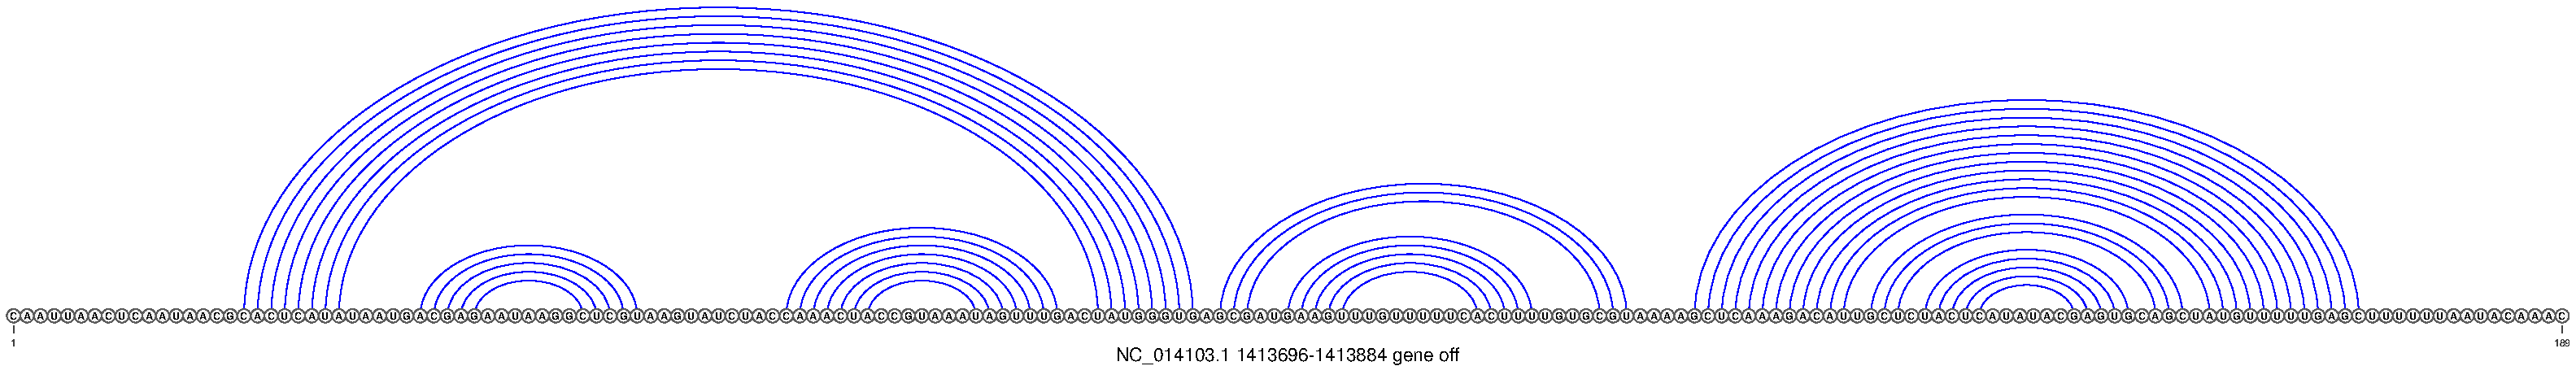
\includegraphics[width=.9\textwidth]{Figures/Ribofinder/NC_014103_1_1413696_1413884_OFF.pdf}
\end{subfigure} \\
\medskip
\begin{subfigure}[h]{\textwidth}
\centering
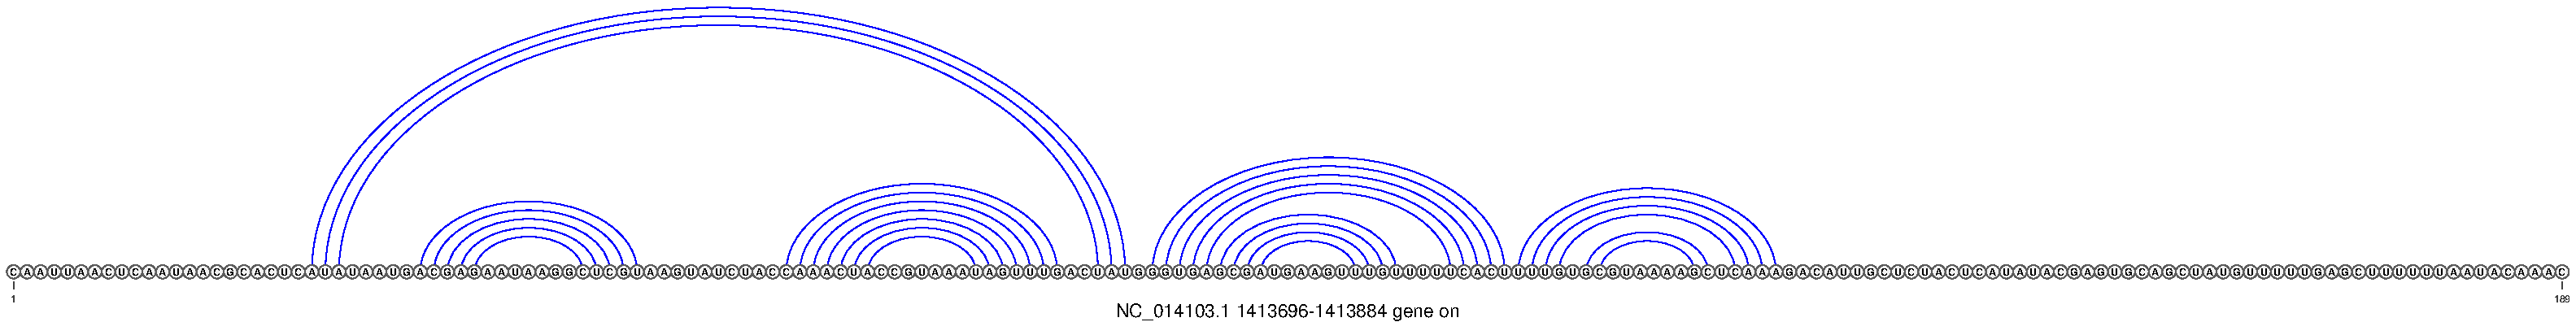
\includegraphics[width=.9\textwidth]{Figures/Ribofinder/NC_014103_1_1413696_1413884_ON.pdf}
\end{subfigure}
\caption[Structures for the putative \rb located upstream of the xpt gene in {\em B. megaterium} DSM$319$]{The computationally predicted \rb located upstream of the xpt
gene in {\em B. megaterium} DSM$319$ (NC\_$014103.1$ $1413696$--$1413884$).
{\em Top:} The gene `off' conformation. {\em Bottom:} The gene `on' conformation.}
\label{fig:figure:NC_014103_1_1413696_1413884}
\end{figure}
\medskip

\begin{figure}[!ht]
\centering
\begin{subfigure}[h]{\textwidth}
\centering
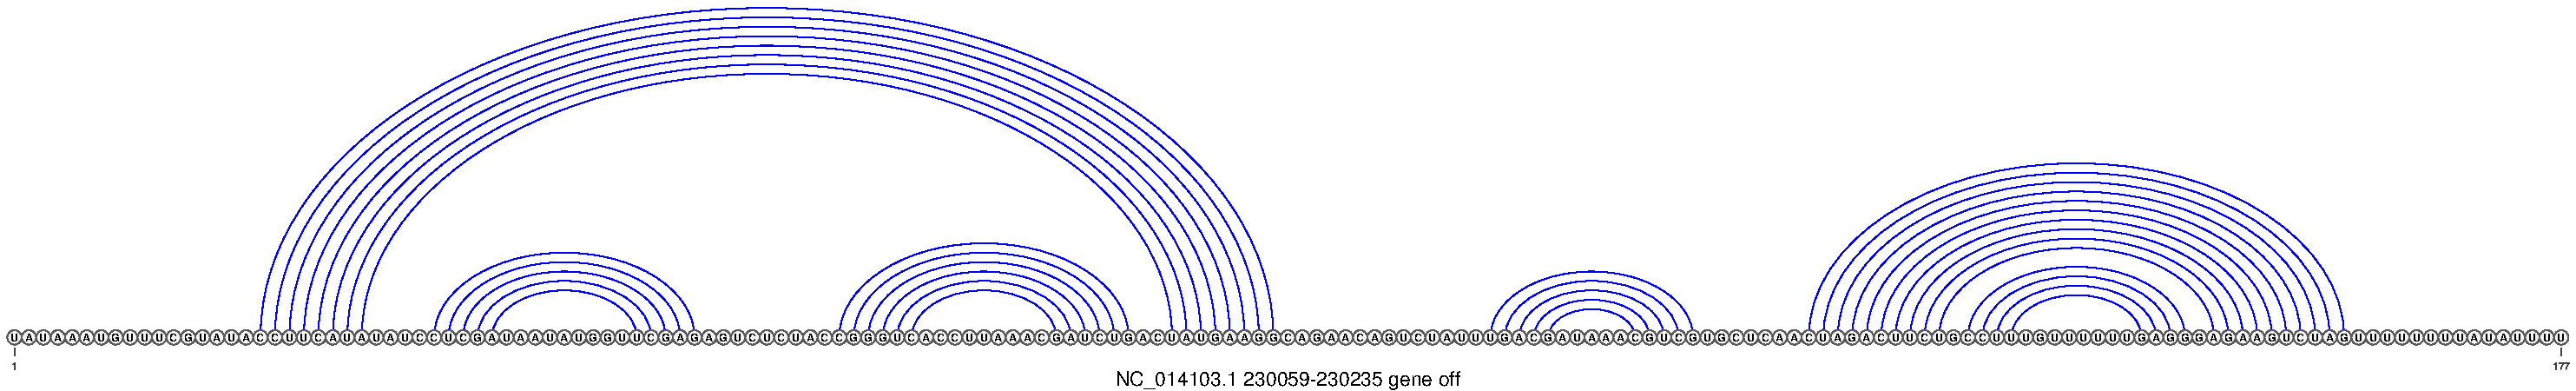
\includegraphics[width=.9\textwidth]{Figures/Ribofinder/NC_014103_1_230059_230235_OFF.pdf}
\end{subfigure} \\
\medskip
\begin{subfigure}[h]{\textwidth}
\centering
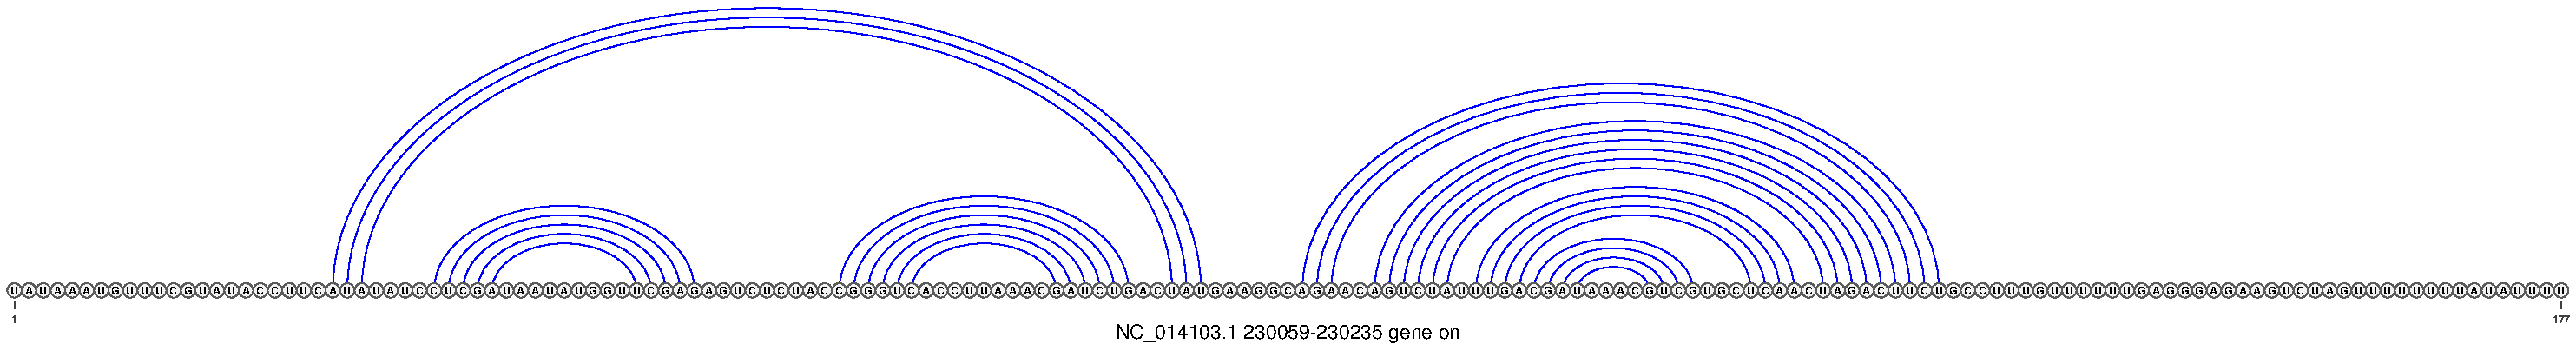
\includegraphics[width=.9\textwidth]{Figures/Ribofinder/NC_014103_1_230059_230235_ON.pdf}
\end{subfigure}
\caption[Structures for the putative \rb located upstream of the GMP synthase gene in {\em B. megaterium} DSM$319$]{The computationally predicted \rb located upstream of the GMP synthase
gene in {\em B. megaterium} DSM$319$ (NC\_$014103.1$ $230059$--$230235$).
{\em Top:} The gene `off' conformation. {\em Bottom:} The gene `on' conformation.}
\label{fig:figure:NC_014103_1_230059_230235}
\end{figure}
\medskip

\begin{figure}[!ht]
\centering
\begin{subfigure}[h]{\textwidth}
\centering
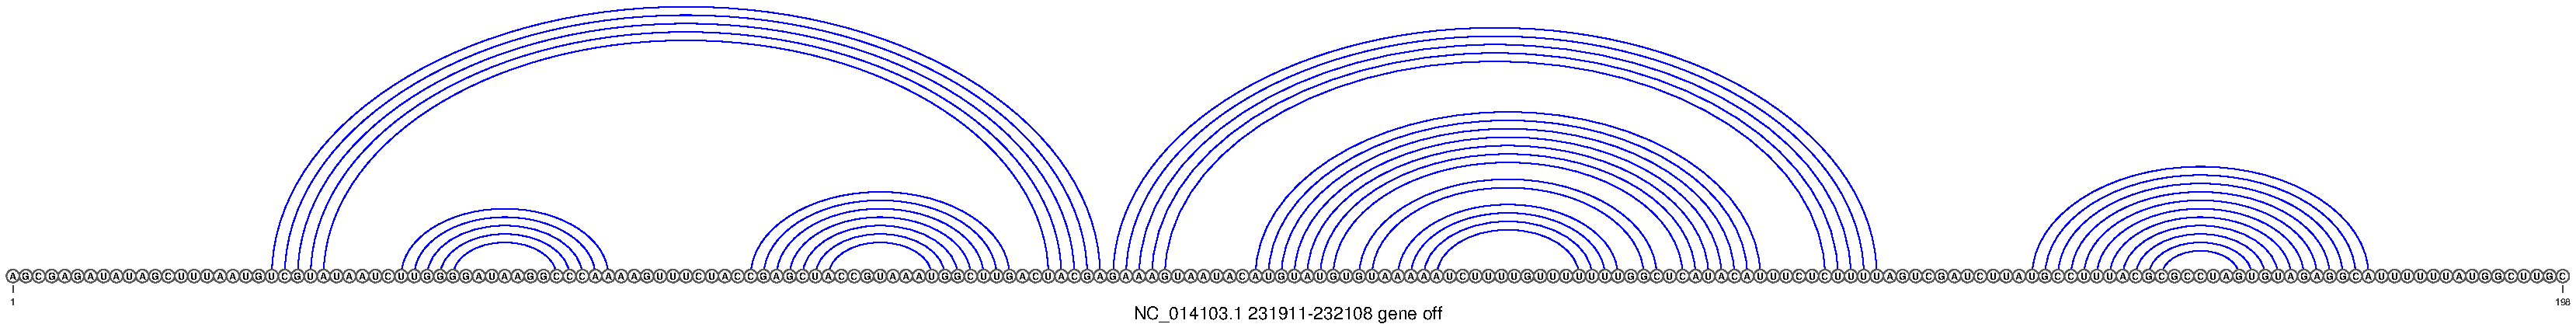
\includegraphics[width=.9\textwidth]{Figures/Ribofinder/NC_014103_1_231911_232108_OFF.pdf}
\end{subfigure} \\
\medskip
\begin{subfigure}[h]{\textwidth}
\centering
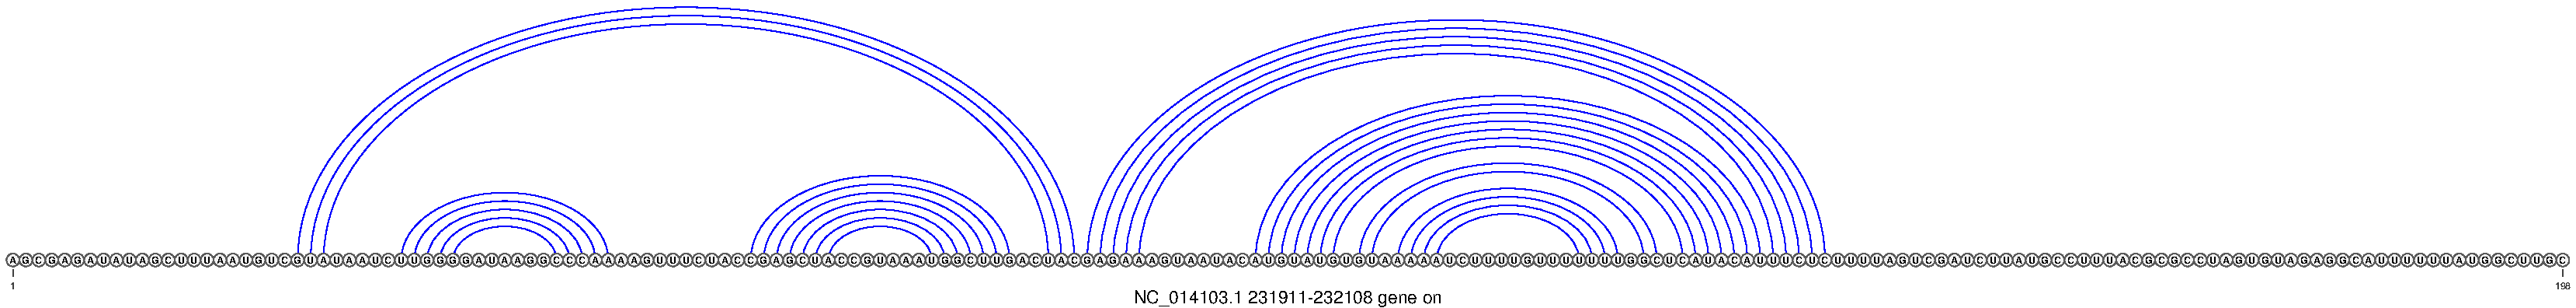
\includegraphics[width=.9\textwidth]{Figures/Ribofinder/NC_014103_1_231911_232108_ON.pdf}
\end{subfigure}
\caption[Structures for the putative \rb located upstream of the guanine permease gene in {\em B. megaterium} DSM$319$]{The computationally predicted \rb located upstream of the guanine permease
gene in {\em B. megaterium} DSM$319$ (NC\_$014103.1$ $231911$--$232108$).
{\em Top:} The gene `off' conformation. {\em Bottom:} The gene `on' conformation.}
\label{fig:figure:NC_014103_1_231911_232108}
\end{figure}
\medskip

\begin{figure}[!ht]
\centering
\begin{subfigure}[h]{\textwidth}
\centering
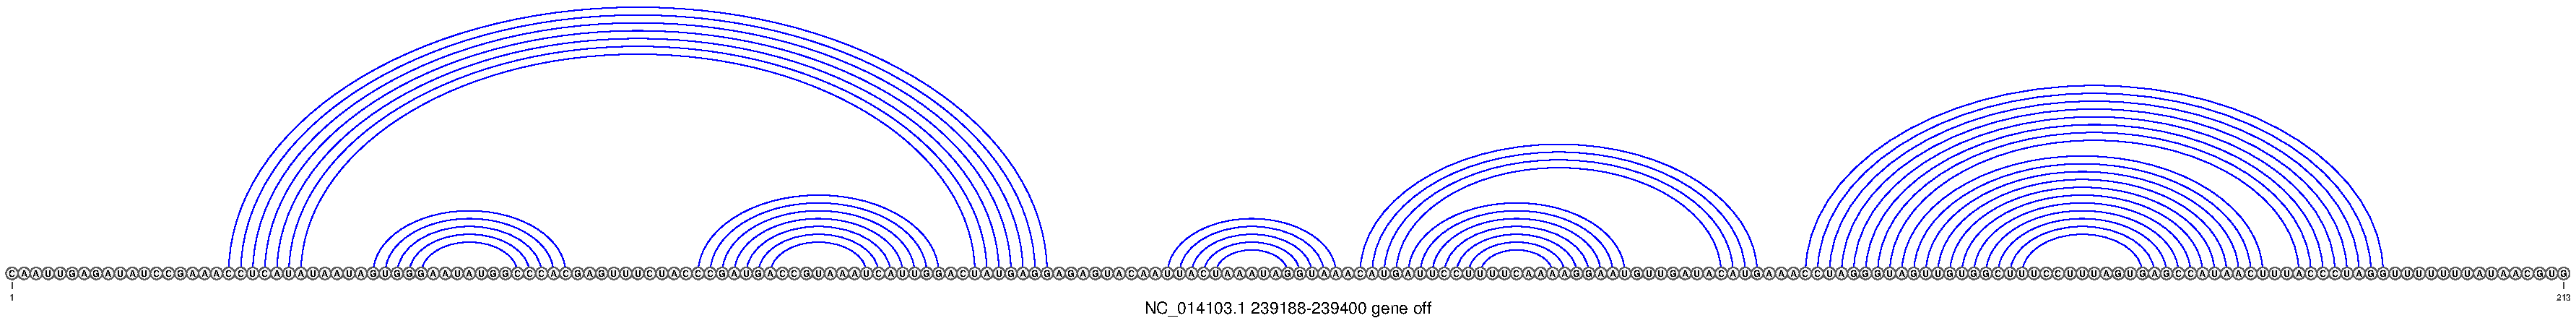
\includegraphics[width=.9\textwidth]{Figures/Ribofinder/NC_014103_1_239188_239400_OFF.pdf}
\end{subfigure} \\
\medskip
\begin{subfigure}[h]{\textwidth}
\centering
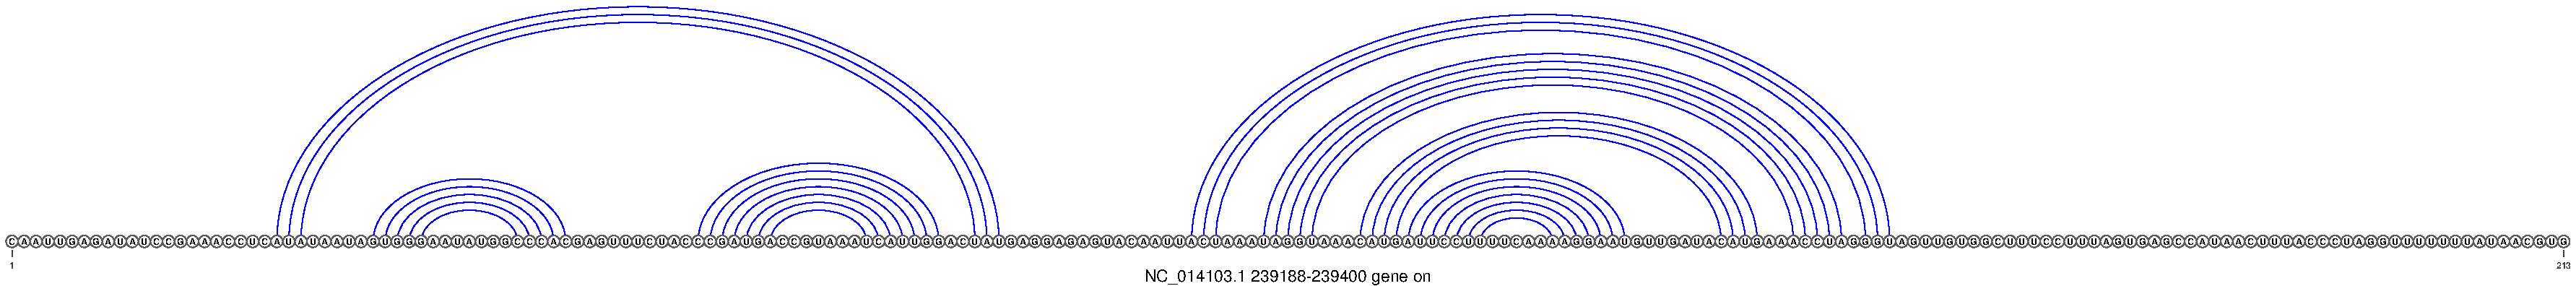
\includegraphics[width=.9\textwidth]{Figures/Ribofinder/NC_014103_1_239188_239400_ON.pdf}
\end{subfigure}
\caption[Structures for the putative \rb located upstream of the N5-carboxy\-amino\-imidazole gene in {\em B. megaterium} DSM$319$]{The computationally predicted \rb located upstream of the
N5-carboxy\-amino\-imidazole
gene in {\em B. megaterium} DSM$319$ (NC\_$014103.1$ $239188$--$239400$).
{\em Top:} The gene `off' conformation. {\em Bottom:} The gene `on' conformation.}
\label{fig:figure:NC_014103_1_239188_239400}
\end{figure}
